\documentclass[11pt,a4paper]{amsart}
\usepackage[utf8]{inputenc}
\usepackage[T1]{fontenc}
\usepackage{lmodern}
\usepackage[expansion=false]{microtype}
\usepackage{amsmath,amssymb,amsthm}
\usepackage{booktabs}
\usepackage{graphicx}
\usepackage[margin=2.3cm]{geometry}
\usepackage{xcolor}
\usepackage[colorlinks=true,linkcolor=blue!50!black,citecolor=blue!50!black,urlcolor=blue!50!black]{hyperref}

\newtheorem{theorem}{Theorem}[section]
\newtheorem{proposition}[theorem]{Proposition}
\newtheorem{lemma}[theorem]{Lemma}
\newtheorem*{theoremA}{Theorem A}
\newtheorem*{theoremB}{Theorem B}
\theoremstyle{remark}
\newtheorem{remark}[theorem]{Remark}

\newcommand{\F}{\mathbb{F}}
\newcommand{\Fq}{\mathbb{F}_q}
\newcommand{\Tr}{\mathrm{Tr}}
\newcommand{\lcm}{\mathrm{lcm}}
\newcommand{\bd}{\mathbf{d}}
\newcommand{\ba}{\mathbf{a}}
\newcommand{\MKB}{\cite{MKB}}

\title[Prescribed traces in intermediate extensions: an audit]{\textbf{Normal and primitive normal elements
with prescribed traces in intermediate extensions: counterexamples, corrected main term, and
improved thresholds}}
\author{Ruqing Chen}
\address{GUT Geoservice Inc., Montreal, Canada}
\email{ruqing@hotmail.com}
\date{November 17, 2026}
\subjclass[2020]{12E20, 11T24, 11T30}
\keywords{finite fields, normal elements, primitive elements, prescribed trace, character sums}

\begin{document}
\begin{abstract}
We audit the paper of Mazumder, Kapetanakis and Basnet (Finite Fields Appl.\ 110 (2026) 102745) on normal and
primitive normal elements of $\F_{q^m}$ with prescribed traces over several intermediate fields
$\F_{q^{d_1}},\dots,\F_{q^{d_k}}$. Its enumeration of normal elements is correct, and we confirm it exhaustively
in $36$ cases. The existence results need repair. The main term of the character sum is evaluated without a
factor $q^{D}$, $D=d_1+\dots+d_k$, so the sufficient condition is printed with exponent $m/2-\lambda-D$ where
$m/2-\lambda$ is correct. The final theorem omits the hypothesis that the prescribed traces be normal, and is
then false for exactly $q^{\lambda}-\Phi(g)>0$ trace tuples for every choice of parameters. Two of its
threshold proofs rest on inequalities that fail for all large $m$. The reduction of non-coprime degrees to
coprime ones by a change of base field is invalid, and the case $\lcm(d_i)<m$ is not proved. We prove the
corrected condition and derive new thresholds: for pairwise coprime degrees, a primitive normal element with
any normal admissible traces exists for all $q\ge4$ when $4\le k\le7$ (printed: $q\ge1334,9,7,5$) and for
all $q\ge8003$ when $k=3$ (printed: $q\ge2.27\cdot10^{24072855}$ and $m\ge60$).
\end{abstract}
\maketitle

\section{Introduction}

Let $q$ be a power of a prime $p$, let $m>1$, and write $\Tr_{m/d}$ for the trace
$\F_{q^m}\to\F_{q^d}$. Fix divisors $d_1<\dots<d_k<m$ of $m$, $k\ge2$, with $d_i\nmid d_j$ for $i\ne j$, and
put $\bd=(d_1,\dots,d_k)$,
\[
D=d_1+\dots+d_k,\qquad g=\lcm(x^{d_1}-1,\dots,x^{d_k}-1)\in\Fq[x],\qquad\lambda=\lambda(\bd)=\deg g .
\]
A tuple $\ba=(a_1,\dots,a_k)$ with $a_i\in\F_{q^{d_i}}$ is \emph{admissible} if
$\Tr_{d_i/e}(a_i)=\Tr_{d_j/e}(a_j)$ for all $i,j$, where $e=\gcd(d_i,d_j)$, and \emph{normal} if every $a_i$
is normal over $\Fq$. By Reis~\cite{Reis} each admissible tuple is the trace tuple
$(\Tr_{m/d_i}(\alpha))_i$ of exactly $q^{m-\lambda}$ elements $\alpha\in\F_{q^m}$, so there are $q^{\lambda}$
admissible tuples. Let $n(\ba)$ and $N(\ba)$ be the numbers of normal, respectively primitive normal,
elements $\alpha\in\F_{q^m}$ (normality is always over $\Fq$) with $\Tr_{m/d_i}(\alpha)=a_i$ for all $i$. As
usual $\Phi(f)=|(\Fq[x]/f)^*|$, and $W(\cdot)$ counts square-free divisors of an integer or monic square-free
divisors of a polynomial over $\Fq$.

The paper \MKB\ determines $n(\ba)$ (its Theorem~3.6), gives a sufficient condition for $N(\ba)>0$
(Theorem~4.1), asserts $N(\ba)>0$ whenever $\lcm(d_1,\dots,d_k)<m$ (Theorem~4.2), and derives explicit
thresholds for pairwise coprime $d_i$ (Theorem~5.1). We follow the numbering of the authors' post-referee text
arXiv:2510.14840v1; no corrigendum to \MKB\ is registered with Crossref. Our findings are as follows.

\begin{enumerate}
\item[(F1)] \emph{Section~3 is correct.} Theorem~3.6, $n(\ba)=\Phi(x^m-1)/\Phi(g)$ for normal admissible
$\ba$, holds for all $q$ and $m$; the standing hypotheses $\gcd(m,q)=1$ and ``$m$ not a prime power'' are
not needed (Proposition~\ref{prop:count}).
\item[(F2)] \emph{The main term in Section~4 is wrong by a factor $q^{D}$.} Theorem~4.1 is true, but with
exponent $m/2-\lambda$ in place of $m/2-\lambda-D$ (Theorem~A). Every statement of the form ``(4.1) does not
hold for any $q$'' in Section~5 is an artefact of this slip.
\item[(F3)] \emph{Theorem~5.1 is false as printed.} It assumes $\ba$ admissible but not normal; for every
$(q,m,\bd)$ exactly $q^{\lambda}-\Phi(g)>0$ admissible tuples have $N(\ba)=0$
(Proposition~\ref{prop:nonnormal}).
\item[(F4)] \emph{Two threshold proofs in Theorem~5.1 are invalid}: the inequality used for $k=4$ fails at
$q=1334$ for every $m>210$ we tested, and the one used for $k=3$ is false for every $q$ once $m\ge62$.
Theorem~B replaces all items with proved and much smaller thresholds.
\item[(F5)] \emph{Theorem~4.2 is not proved.} The indicated argument yields normality over
$\F_{q^{L}}$, $L=\lcm(d_i)$, not over $\Fq$, and the two differ on explicit elements
(Proposition~\ref{prop:lcm}). We prove the statement when $m/L$ is a power of $p$ and whenever Theorem~A
applies; it holds in all cases we could enumerate.
\item[(F6)] \emph{The coprimality hypothesis cannot be removed by base change.} Remark~(1) of Section~5
replaces $q$ by $q^{\gcd(d_1,d_2)}$; this changes both the set of normal tuples and the set of normal
elements (Proposition~\ref{prop:basechange}). Non-coprime degrees must be treated over $\Fq$, as Theorem~A
does.
\end{enumerate}
We found no counterexample to an existence statement once $\ba$ is assumed normal: in all $36$ triples
$(q,m,\bd)$ within reach of exhaustive enumeration, $N(\ba)>0$ for every normal admissible $\ba$.

\section{The count of normal elements and the missing hypothesis}

\begin{proposition}\label{prop:count}
For all $q$, $m$, $\bd$ as above and every admissible $\ba$,
\[
n(\ba)=\begin{cases}\Phi(x^m-1)/\Phi(g),&\ba\text{ normal},\\ 0,&\text{otherwise,}\end{cases}
\]
and exactly $\Phi(g)$ of the $q^{\lambda}$ admissible tuples are normal.
\end{proposition}
\begin{proof}
If $\alpha$ is normal then so is $\Tr_{m/d}(\alpha)=L_{(x^m-1)/(x^d-1)}(\alpha)\in\F_{q^d}$ \cite[Lemma~3.1]{MKB};
the proof there uses no hypothesis on $q$ or $m$. This gives the second line. For the first, fix a normal
$\gamma\in\F_{q^m}$; the normal elements are the $L_F(\gamma)$ with $F\in(\Fq[x]/(x^m-1))^*$, and
$a_i=L_{h_i}(\Tr_{m/d_i}(\gamma))$ with $h_i$ a unit modulo $x^{d_i}-1$. Then $\Tr_{m/d_i}(L_F(\gamma))=a_i$
if and only if $F\equiv h_i\pmod{x^{d_i}-1}$. Admissibility says $h_i\equiv h_j$ modulo
$\gcd(x^{d_i}-1,x^{d_j}-1)=x^{\gcd(d_i,d_j)}-1$, because $\Tr_{m/\gcd(d_i,d_j)}(\gamma)$ is normal; in the
principal ideal domain $\Fq[x]$ pairwise compatible congruences have a solution, unique modulo $g$, and it is
a unit modulo $g$. Reduction $(\Fq[x]/(x^m-1))^*\to(\Fq[x]/g)^*$ is onto \cite[Lemma~3.3]{MKB}, with fibres of size
$\Phi(x^m-1)/\Phi(g)$. This is the argument of \cite[Theorem~3.6]{MKB}; no step uses $p\nmid m$. Finally the
$\Phi(x^m-1)$ normal elements are spread evenly over the normal admissible tuples, so there are $\Phi(g)$ of
these.
\end{proof}

\begin{proposition}[Theorem~5.1 of \MKB\ as printed]\label{prop:nonnormal}
Theorem~5.1 of \MKB\ asks only that $\ba$ be $\bd$-admissible. For every $q$, every $m$ and every $\bd$ there
are exactly $q^{\lambda}-\Phi(g)\ge1$ admissible tuples $\ba$ with $N(\ba)=n(\ba)=0$; the zero tuple is one of
them. Hence each of the items \textup{(i)--(iii)} of that theorem is false as stated, for every admitted
$q$, and becomes meaningful only for normal $\ba$, as in Theorems~4.1 and~4.2.
\end{proposition}
\begin{proof}
Immediate from Proposition~\ref{prop:count}, since $\Phi(g)<q^{\deg g}=q^{\lambda}$.
\end{proof}

For instance, for $q=2$, $m=6$, $\bd=(2,3)$ there are $16$ admissible pairs, $6$ of them normal; each normal
pair is the trace pair of $4$ normal elements, $3$ of them primitive, and none of the other $10$ pairs is the
trace pair of a normal element, although $5$ of them are trace pairs of primitive elements. Table~\ref{tab:ex}
and Figure~\ref{fig}(a) record the same pattern in all enumerated cases.

\begin{table}[t]
\centering\small
\begin{tabular}{@{}rrlrrrl@{}}
\toprule
$q$ & $m$ & $\bd$ & $q^{\lambda}$ & $\Phi(g)$ & $n(\ba)$ & $N(\ba)$\\
\midrule
$2$ & $6$ & $(2,3)$ & $16$ & $6$ & $4$ & $3$\\
$7$ & $6$ & $(2,3)$ & $2401$ & $1296$ & $36$ & $8$--$17$\\
$13$ & $6$ & $(2,3)$ & $28561$ & $20736$ & $144$ & $26$--$55$\\
$3$ & $10$ & $(2,5)$ & $729$ & $320$ & $80$ & $30$--$40$\\
$3$ & $12$ & $(3,4)$ & $729$ & $288$ & $729$ & $217$--$239$\\
$4$ & $12$ & $(4,6)$ & $65536$ & $27648$ & $256$ & $84$--$123$\\
$2$ & $15$ & $(3,5)$ & $128$ & $45$ & $225$ & $185$--$191$\\
$2$ & $18$ & $(6,9)$ & $4096$ & $1512$ & $64$ & $27$--$44$\\
$2$ & $21$ & $(3,7)$ & $512$ & $147$ & $3969$ & $3353$--$3385$\\
$2$ & $22$ & $(2,11)$ & $4096$ & $2046$ & $1024$ & $630$--$650$\\
$2$ & $24$ & $(6,8)$ & $4096$ & $1536$ & $4096$ & $1553$--$1667$\\
\bottomrule
\end{tabular}
\medskip
\caption{Exhaustive enumeration in $\F_{q^m}$ (a selection of the $36$ cases): number $q^{\lambda}$ of
admissible tuples, number $\Phi(g)$ of normal ones, the common value $n(\ba)=\Phi(x^m-1)/\Phi(g)$ on normal
tuples, and the range of $N(\ba)$ over normal tuples. On the remaining $q^{\lambda}-\Phi(g)$ admissible tuples
$n(\ba)=N(\ba)=0$.}\label{tab:ex}
\end{table}

\section{The corrected sufficient condition}

Put $\theta=\varphi(q^m-1)/(q^m-1)$ and $\Theta=\Phi(x^m-1)/q^m$.

\begin{theoremA}
For all $q$, $m$, $\bd$ and every normal admissible $\ba$,
\begin{equation}\label{eq:A}
\Bigl|\,N(\ba)-\theta\,\frac{\Phi(x^m-1)}{\Phi(g)}\Bigr|\le
\theta\,\Theta\,q^{m/2}\bigl(W(q^m-1)-1\bigr)W(x^m-1).
\end{equation}
In particular $N(\ba)>0$ whenever
\begin{equation}\label{eq:cond}
q^{\,m/2-\lambda(\bd)}\ \ge\ W(q^m-1)\,W(x^m-1).
\end{equation}
\end{theoremA}
\begin{proof}
Expanding the characteristic functions of primitivity, normality and prescribed traces as in
\cite[Section~4]{MKB} gives
\[
\frac{q^{D}N(\ba)}{\theta\,\Theta}=S_1+S_2 ,
\]
where $S_1$ collects the terms with trivial multiplicative character and $S_2$ the others; the factor $q^{D}$
comes from the $k$ trace conditions, each contributing $q^{-d_i}\sum_{c\in\F_{q^{d_i}}}$. By the same
expansion without the primitivity factor, $S_1=q^{D}n(\ba)/\Theta$, so Proposition~\ref{prop:count} gives
\[
S_1=\frac{q^{D}\,\Phi(x^m-1)}{\Phi(g)\,\Theta}=\frac{q^{D+m}}{\Phi(g)}>q^{D+m-\lambda}.
\]
In $S_2$ each Gauss sum has modulus $q^{m/2}$ or vanishes, there are $q^{D}$ choices of
$(c_1,\dots,c_k)$, and the sums over characters of given orders cancel the denominators, whence
$|S_2|\le q^{D+m/2}(W(q^m-1)-1)W(x^m-1)$, exactly as in \MKB. Multiplying by $\theta\Theta q^{-D}$ gives
\eqref{eq:A}; since $\Phi(g)<q^{\lambda}$, \eqref{eq:cond} makes $S_1+S_2$ positive.
\end{proof}

\begin{remark}\label{rem:slip}
In \MKB\ the value $S_1=q^{m}/(\Phi(g)\theta)$ is used: the normalising factor $q^{D}$ on the left is not
carried to $S_1$, while it is kept in the bound for $S_2$. The Gauss sum bound $q^{m/2}$ is correct. The
printed condition~(4.1), $q^{m/2-\lambda-D}\ge W(q^m-1)W(x^m-1)$, is therefore a valid but needlessly strong
sufficient condition; its exponent is too small by $D\ge5$. This matters in Section~5 of \MKB, where the
cases $m\in\{30,42\}$ for $k=3$, and $(d_1,d_2)=(7,8)$, $d_1=6$ with $7\le d_2\le11$, and $d_1\in\{3,4,5\}$
for $k=2$, are set aside because ``(4.1) does not hold for any prime power $q$''. With the correct exponent
all of them are covered for large $q$ except $(3,4)$; see Figure~\ref{fig}(b). The last exclusion is also
wrong on its own terms: for $d_1=5$ and coprime $d_2\ge19$ the printed exponent with $m=5d_2$ is $(d_2-18)/2>0$.
In the enumerated cases $N(\ba)$ stays close to the main term of \eqref{eq:A}: for $q=2$, $m=24$,
$\bd=(3,8)$ it lies between $6423$ and $6534$ for all $384$ normal pairs, the main term being $6480$.
\end{remark}

\section{Corrected thresholds}

Let $P_j$ be the product of the first $j$ primes, and $C_\nu=\prod_{p\le2^\nu}2p^{-1/\nu}$, so that
$W(n)\le C_\nu n^{1/\nu}$ \cite{CH2}; we recomputed $C_{11}=4.2445\cdot10^{14}$,
$C_{12}=1.0573\cdot10^{24}$ and $C_{31}=2.4015\cdot10^{1553069}$, in agreement with \cite[Lemma~2.7]{MKB}.

\begin{theoremB}
Let $d_1<\dots<d_k$ be pairwise coprime integers $\ge2$, $k\ge2$, let $m$ be any proper multiple of
$\lcm(d_i)=d_1\cdots d_k$ or this product itself, and let $\ba$ be a normal admissible tuple. Then
$N(\ba)>0$ in each of the following cases:
\begin{enumerate}
\item[(i)] $k\in\{4,5,6,7\}$ and $q\ge4$;
\item[(ii)] $k=3$ and $q\ge8003$ (including $m=30$ and $m=42$);
\item[(iii)] $k=2$, $(d_1-2)(d_2-2)>2$, that is $d_1\ge3$ and $(d_1,d_2)\ne(3,4)$, and $q\ge q_0(m)$; for
example $q\ge192$ suffices for $(d_1,d_2)=(8,9)$, $q\ge289$ for $(5,19)$, and $q\ge795$ for $(7,8)$.
\end{enumerate}
\end{theoremB}
\begin{proof}
Here $\lambda=D-k+1$. By Theorem~A, $W(q^m-1)<C_\nu q^{m/\nu}$ and the bound
$W(x^m-1)\le2^{b}$, $b=\tfrac12(m+\gcd(m,q-1))$, of Lenstra and Schoof~\cite{LS}, it suffices to find $\nu$ with
\begin{equation}\label{eq:B}
\Bigl(\frac m2-D+k-1-\frac m\nu\Bigr)\log q\ \ge\ \log C_\nu+b\log2 .
\end{equation}
\emph{Case} (iii). The exponent $m/2-D+1\ge\tfrac12(d_1-2)(d_2-2)-1$ is positive; fix $\nu$ larger than $m$
divided by it and use $b\le m$: \eqref{eq:B} holds for large $q$. The explicit values come from
$\nu\le14$.

\emph{Cases} (i), (ii). Write $n_0=d_1\cdots d_k\mid m$. First, $d_k\le n_0/P_{k-1}$ and
$d_i<d_{k-1}<(n_0/P_{k-2})^{1/2}$ for $i<k-1$, because $d_{k-1}^2<d_{k-1}d_k\le n_0/P_{k-2}$; hence
\begin{equation}\label{eq:D}
D<\frac{m}{P_{k-1}}+(k-1)\Bigl(\frac{m}{P_{k-2}}\Bigr)^{1/2}.
\end{equation}
With $b\le m$ the difference of the two sides of \eqref{eq:B} is, for a fixed tuple and $\nu$, linear in $m$
and increasing in $q$, so it is enough to treat $m=n_0$ for the smallest $q$, with a slope
$(\tfrac12-\tfrac1\nu)\log q-\log2\ge0$; and after inserting \eqref{eq:D} it is a convex function of $m$
alone. We enumerated all tuples with $n_0\le M_0$ ($181624$ triples for $M_0=10^5$; $92412$ quadruples for
$M_0=2\cdot10^5$; $77887$, $15961$ and $12898$ tuples for $k=5,6,7$ and $M_0=10^6$, $3\cdot10^6$,
$3\cdot10^7$) and checked \eqref{eq:B} with the exact $D$ and some $3\le\nu\le14$, and checked that the convex
bound and its derivative are non-negative at $m=M_0$. With $b\le m$ this gives (ii), the extremal case being
$\bd=(2,3,5)$, $m=30$, $\nu=8$, and it gives $q\ge11$ for $k=4$ and $q\ge6$ for $k=5,6,7$. For the remaining
prime powers $4\le q\le9$ we used the exact $b$ at $m=n_0$, the bound $b\le\tfrac12(m+q-1)$ at the proper
multiples of $n_0$, where the difference is again linear in $m$, and $b\le\tfrac34m$ for $m>M_0\ge q$; all
checks succeed for $q\ge4$ and fail for $q\in\{2,3\}$.
\end{proof}

\begin{table}[t]
\centering\footnotesize
\begin{tabular}{@{}llll@{}}
\toprule
$k$ & printed in \cite[Theorem~5.1]{MKB} & printed proof & proved here\\
\midrule
$2$ & $q$ large; $d_1\ge8$; $d_1=7$, $d_2\ne8$; $d_1=6$, $d_2\ge13$ & incomplete list &
$q$ large; $d_1\ge3$, $\bd\ne(3,4)$\\
$3$ & $q\ge2.2660\cdot10^{24072855}$, $m\ge60$ & invalid for $m\ge62$ & $q\ge8003$, all $m$\\
$4$ & $q\ge1334$ & invalid for $m>210$ & $q\ge4$\\
$5,\,6,\,7$ & $q\ge9$, $q\ge7$, $q\ge5$ & valid if $m=d_1\cdots d_k$ & $q\ge4$\\
\bottomrule
\end{tabular}
\medskip
\caption{Thresholds for pairwise coprime $d_1,\dots,d_k$ and normal admissible $\ba$.}\label{tab:thr}
\end{table}

\begin{remark}[The printed proofs]\label{rem:proofs}
For $k=4$, \MKB\ bounds $D\le k\lfloor m/k!\rfloor$ and claims
$q^{m/2-8\lfloor m/24\rfloor+3}\ge C_{11}q^{m/11}2^{m}$ for all $m\ge210$ and $q\ge1334$. This holds at
$m=210$ (it needs $q\ge1333.9$) but needs $q\ge2249$ at $m=330$ and $q>2^{66/5}\approx9410$ as $m\to\infty$;
at $q=1334$ it fails for $342$ of the $343$ integers $210\le m<5000$ with at least four prime factors. For
$k=3$ the bound $D\le m/4$ is correct for $m\ge60$ (the intermediate claim $d_3\le m/10$ is not: take
$\bd=(2,3,13)$), but the resulting condition $q^{2}\ge C_{31}q^{m/31}2^{m}$ is false for every $q$ as soon as
$m\ge62$; the printed threshold is its value at $m=60$. In both cases the loss is in replacing the true
exponent by its minimum before comparing with a right-hand side that grows with $m$. The printed
inequalities for $k=5,6,7$ do hold. All items of Theorem~5.1 are proved in \MKB\ only for
$m=d_1\cdots d_k$, the case $\lcm(d_i)<m$ being referred to Theorem~4.2; Theorem~B does not need this
reduction. We also checked \cite[Lemma~2.9]{MKB} for $3\le t\le10^{6}$. For $k\ge4$ and $q\in\{2,3\}$, and for
$k=3$ and $q<8003$, the question remains open; these fields ($m\ge30$) are beyond exhaustive search here.
\end{remark}

\section{\texorpdfstring{The case $\lcm(d_i)<m$ and the change of base field}{The case lcm(d\_i) < m and the change of base field}}

According to Theorem~4.2 of \MKB, $N(\ba)>0$ for every normal admissible $\ba$ if $L=\lcm(d_1,\dots,d_k)<m$; this is
called ``an immediate consequence'' of \cite{Reis} and the theorem of Cohen and Hachenberger~\cite{CH}, the proof
being omitted. The natural argument takes $\beta\in\F_{q^{L}}$ with $\Tr_{L/d_i}(\beta)=a_i$ and then a
primitive $\alpha\in\F_{q^m}$, normal over $\F_{q^{L}}$, with $\Tr_{m/L}(\alpha)=\beta$.

\begin{proposition}\label{prop:lcm}
\textup{(a)} If $m/L$ is a power of $p$, then $N(\ba)>0$ for every normal admissible $\ba$.

\textup{(b)} In general a primitive element that is normal over $\F_{q^{L}}$, has normal admissible traces
$a_i$, and has a trace $\beta$ over $\F_{q^L}$ that is normal over $\Fq$, need not be normal over $\Fq$:
for $q=3$, $m=12$, $\bd=(2,3)$, $L=6$ there are $73872$ such elements and $8448$ of them are not normal over
$\F_3$; for $q=2$, $m=18$, $\bd=(2,3)$, $L=6$ the numbers are $50976$ and $828$.
\end{proposition}
\begin{proof}
(a) Since $d_i\nmid d_j$, each $d_i$ is a proper divisor of $L$, and Proposition~\ref{prop:count} in
$\F_{q^{L}}$ gives $\beta\in\F_{q^{L}}$, normal over $\Fq$, with $\Tr_{L/d_i}(\beta)=a_i$. As $\beta\ne0$,
Cohen's theorem~\cite{C90} gives a primitive $\alpha\in\F_{q^m}$ with $\Tr_{m/L}(\alpha)=\beta$. Now
$x^m-1=(x^{L}-1)^{m/L}$, so every irreducible $P\mid x^m-1$ divides $x^{L}-1$ and
$L_{(x^m-1)/P}(\alpha)=L_{(x^{L}-1)/P}(\beta)\ne0$; thus $\alpha$ is normal over $\Fq$. (b) is by
enumeration.
\end{proof}

So Theorem~4.2 is proved when $m/L$ is a power of $p$ and when \eqref{eq:cond} holds, and is otherwise
open. In every enumerated case with $L<m$ ($\bd=(2,3)$ for $(q,m)=(2,12)$, $(3,12)$, $(4,12)$, $(2,18)$, $(2,24)$; $(2,5)$ for
$(2,20)$; $(3,4)$ and $(4,6)$ for $(2,24)$) we found $N(\ba)>0$ for all normal $\ba$.

Remark~(1) in Section~5 of \MKB\ asserts that for $k=2$ the condition $\gcd(d_1,d_2)=1$ ``is not
restrictive'': with $d=\gcd(d_1,d_2)$ and $Q=q^{d}$ one has $\F_{q^{d_i}}=\F_{Q^{t_i}}$, $t_i=d_i/d$ coprime.
A result over $\F_Q$ needs $\ba$ normal over $\F_Q$ and returns elements normal over $\F_Q$; neither property
agrees with its counterpart over $\Fq$.

\begin{proposition}\label{prop:basechange}
\textup{(a)} Let $q=2$, $m=12$, $\bd=(4,6)$, $Q=4$. Of the $96$ normal admissible pairs, $48$ are not normal
over $\F_4$. No element normal over $\F_4$ has such a pair as traces, while $n(\ba)=16$ and $N(\ba)\ge5$.
In $\F_{2^{12}}$, $1536$ elements are normal over $\F_2$, $1728$ over $\F_4$, and $768$ over both. For
$q=2$, $m=20$, $\bd=(4,10)$ the same happens for $240$ of the $1920$ normal admissible pairs.

\textup{(b)} Let $q=5$, $m=12$, $\bd=(4,6)$, $Q=25$, so that $p\nmid m$. In
$\F_{5^{12}}=\F_5[t]/(t^{12}+t^{11}+t^{10}+t^{9}+2t^{8}+4t^{7}+4t^{6}+2t^{4}+2t^{3}+t^{2}+t+2)$ the element
\[
\alpha=3t^{10}+4t^{8}+4t^{7}+3t^{6}+2t^{5}+4t^{4}+t^{2}+2
\]
is primitive and normal over $\F_{25}$, its traces over $\F_{5^{4}}$ and $\F_{5^{6}}$ are normal over $\F_5$
and over $\F_{25}$, and $\alpha$ is not normal over $\F_5$: it is annihilated by $L_f$ with
$f=(x^{12}-1)/(x^{2}+2x+4)$.
\end{proposition}
\begin{proof}
By computation. The mechanism in (b) is that $x^{2}+2x+4$ and $x^{2}+3x+4$, the factors of $x^{12}-1$ over
$\F_5$ dividing neither $x^{4}-1$ nor $x^{6}-1$, are not seen by the traces, and the two corresponding
components of $\F_{5^{12}}$ as an $\F_5[x]$-module do not coincide with the two components attached to the
factors $y-\omega^{\pm1}$ of $y^{6}-1$ over $\F_{25}$ ($\omega$ of order $6$) of the $\F_{25}[y]$-module,
$y=x^{2}$; an element may vanish in one of the former and in neither of the latter.
\end{proof}

Non-coprime degrees are nevertheless within reach: Theorem~A makes no coprimality assumption, and for $k=2$
it gives $N(\ba)>0$ for large $q$ as soon as $m/2>d_1+d_2-\gcd(d_1,d_2)$.

\begin{figure}[t]
\centering
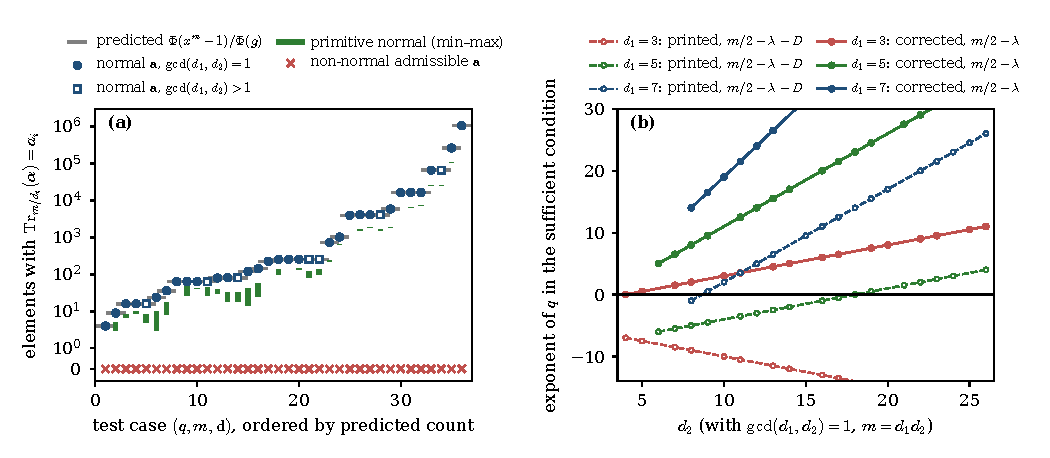
\includegraphics[width=\textwidth]{fig_intermediate_traces_audit.pdf}
\caption{(a) Exhaustive counts for the $36$ enumerated triples $(q,m,\bd)$, $k=2$: the number of normal
elements with a given normal admissible trace pair equals $\Phi(x^m-1)/\Phi(g)$ whether or not
$\gcd(d_1,d_2)=1$, the number of primitive normal ones is positive, and both vanish for the non-normal
admissible pairs allowed by the printed Theorem~5.1. (b) Exponent of $q$ in the sufficient condition for
$k=2$, $m=d_1d_2$: printed (dashed) and corrected (solid). A positive exponent gives existence for large
$q$.}\label{fig}
\end{figure}

\section{Further remarks, computations and data}\label{sec:verif}

Minor slips in \MKB, none affecting the results: $\theta(q)$ is defined with $q^{n}$ for $q^{m}$ and the final
display of Section~4 has $\Theta(q)$ for $\Theta(x^m-1)$; $\kappa_m$ is introduced as the characteristic
function of normality over $\F_{q^{d}}$ but used over $\Fq$; several traces are written $\Tr_{n/d_i}$ for
$\Tr_{m/d_i}$; and the letter $k$ denotes both the number of fields and the fibre size in Theorem~3.4.

All enumerations were carried out with exact arithmetic in $\F_{q^m}$ for the $36$ triples $(q,m,\bd)$ with
$k=2$, $q\le13$ and $q^{m}\le2^{24}$: $m=6$ ($q\le13$), $m=10$ ($q\le4$), $m=12$ ($q\le4$), and
$m\in\{14,15,18,20,21,22,24\}$ ($q=2$), with all pairs $\bd$ listed in the data. Normality over $\Fq$ was
tested through the linearised cofactors $L_{(x^m-1)/P}$, with $x^m-1$ factored over $\Fq$ via cyclotomic
cosets, and cross-checked on all fields with at most $20000$ elements by the criterion that $x^m-1$ be coprime to
$\sum_i\alpha^{q^{i}}x^{m-1-i}$. In each case we verified Reis's count $q^{m-\lambda}$,
Proposition~\ref{prop:count}, inequality~\eqref{eq:A}, and $N(\ba)>0$ for all normal admissible $\ba$. The
programs, their logs and the data behind the tables and the figure are available at
\url{https://github.com/Ruqing1963/kapetanakis-intermediate-traces-audit} and archived at
\href{https://doi.org/10.5281/zenodo.24345226}{doi:10.5281/zenodo.24345226}.

\section*{Declaration of generative AI and AI-assisted technologies in the manuscript preparation process}
During the preparation of this work the author used Claude (Anthropic) and Gemini (Google) to assist with
writing and running the Python verification scripts, checking symbolic identities and inequalities, and drafting
and editing the LaTeX manuscript. The numerical tables, explicit examples, and finite-range computations were
checked by running the deterministic verification programs described in Section~\ref{sec:verif}, and the author
checked the statements and proofs. After using these tools, the author reviewed and edited the content as needed
and takes full responsibility for the content of the published article.
\begin{thebibliography}{9}
\bibitem{MKB} A.~C. Mazumder, G.~Kapetanakis, D.~K. Basnet, Normal and primitive normal elements with
prescribed traces in intermediate extensions of finite fields, \emph{Finite Fields Appl.} \textbf{110} (2026),
102745, \href{https://doi.org/10.1016/j.ffa.2025.102745}{doi:10.1016/j.ffa.2025.102745}; arXiv:2510.14840.
\bibitem{C90} S.~D. Cohen, Primitive elements and polynomials with arbitrary trace, \emph{Discrete Math.}
\textbf{83} (1990), 1--7.
\bibitem{CH} S.~D. Cohen, D.~Hachenberger, Primitive normal bases with prescribed trace, \emph{Appl. Algebra
Engrg. Comm. Comput.} \textbf{9} (1999), 383--403.
\bibitem{CH2} S.~D. Cohen, S.~Huczynska, The strong primitive normal basis theorem, \emph{Acta Arith.}
\textbf{143} (2010), 299--332.
\bibitem{LS} H.~W. Lenstra, Jr., R.~J. Schoof, Primitive normal bases for finite fields, \emph{Math. Comp.}
\textbf{48} (1987), 217--231.
\bibitem{Reis} L.~Reis, Counting solutions of special linear equations over finite fields, \emph{Finite
Fields Appl.} \textbf{68} (2020), 101759.
\end{thebibliography}
\end{document}
